\documentclass[10pt, aspectratio=169]{beamer}

\usetheme[progressbar=frametitle]{metropolis}

\usepackage[utf8]{inputenc}
\usepackage{lmodern}
\usepackage{appendixnumberbeamer}
\usepackage{xcolor}
\usepackage{subcaption}
\usepackage{tikz}
\usepackage{bm}
\usepackage{booktabs}


\usetikzlibrary{arrows,positioning}

\mode<presentation>
% enable the following row to show notes for training your talk
%\setbeameroption{show notes on second screen}


\definecolor{rwthblue}{RGB}{0,84,159}
\definecolor{rwthmagenta}{RGB}{227,0,102}
\definecolor{rwthyellow}{RGB}{255,237,0}
\definecolor{rwthgreen}{RGB}{87,171,39}
\definecolor{rwthred}{RGB}{204,7,30}

\setbeamercolor{normal text}{fg=rwthblue, bg=white}
\setbeamercolor{alerted text}{fg=rwthmagenta}
\setbeamercolor{example text}{fg=rwthyellow}

\newcommand{\source}[1]{
  \begin{tikzpicture}[remember picture, overlay]
    \node[xshift=0cm, yshift=-.3cm, above=of current page.south] {\footnotesize Source: #1};
  \end{tikzpicture}
}

\title{Long Short-Term Memory}
\subtitle{Joint Proseminar on Machine Learning and Image Processing}
\date{\today}
\author{Fynn Jansen, Leon Benzer}
\institute{Chair of Computer Science 13 (Computer Vision)\\RWTH Aachen}
\makeatletter
\setbeamertemplate{frame footer}{Long Short-Term Memory \hfill Fynn Jansen, Leon Benz, RWTH}
\makeatother

\begin{document}

\maketitle

% ----------------------------------------------------------------

% Contents
\begin{frame}[t]{Contents}
\begin{itemize}
    \item \textbf{Introduction}
    \item Recap
    \item Naive Solution
    \item LSTM Architecture
    \item Variants
    \item GRU
    \item LSTM vs Transformer
    \item Applications
    \item Discussion
    \item Conclusion
\end{itemize}
\end{frame}

%Introduciton
\begin{frame}[t]{Introduction - The importance of Sequence Data}
Data best described by sequences:
\end{frame}

\begin{frame}[t]{Introduction - The importance of Sequence Data}
Data best described by sequences:
\begin{itemize}
    \item Language
\end{itemize}
\end{frame}

\begin{frame}[t]{Introduction - The importance of Sequence Data}
Examples for sequence Data:
\begin{itemize}
    \item Language
    \item Music \& Audio
\end{itemize}
\end{frame}

\begin{frame}[t]{Introduction - The importance of Sequence Data}
Examples for sequence Data:
\begin{itemize}
    \item Language
    \item Music \& Audio
    \item (Stock) prices
\end{itemize}
\end{frame}

\begin{frame}[t]{Introduction - The importance of Sequence Data}
Examples for sequence Data:
\begin{itemize}
    \item Language
    \item Music \& Audio
    \item (Stock) prices
    \item Weather
\end{itemize}
\end{frame}

\begin{frame}[t]{Introduction - The importance of Sequence Data}
Examples for sequence Data:
\begin{itemize}
    \item Language
    \item Music \& Audio
    \item (Stock) prices
    \item Weather
\end{itemize}
\begin{math}\implies\end{math} Real world data often best described by sequences
\end{frame}



% Recap
\begin{frame}[t]{Contents}
\begin{itemize}
    \item Introduction
    \item \textbf{Recap}
    \item Naive Solution
    \item LSTM Architecture
    \item Variants
    \item GRU
    \item LSTM vs Transformer
    \item Applications
    \item Discussion
    \item Conclusion
\end{itemize}
\end{frame}

\begin{frame}[t]{Recap - RNNs}
    
\end{frame}

\begin{frame}{Recap - Unstable Gradients}
    
\end{frame}

% Constant Error Carousel
\begin{frame}[t]{Contents}
\begin{itemize}
    \item Introduction
    \item Recap
    \item \textbf{Naive Solution}
    \item LSTM Architecture
    \item Variants
    \item GRU
    \item LSTM vs Transformer
    \item Applications
    \item Discussion
    \item Conclusion
\end{itemize}
\end{frame}

\begin{frame}[t]{Naive Solution - Constant Error Flow}
    Single Unit Constant Error Carousel:
    \source{Hochreiter et al. 1997}
\end{frame}

\begin{frame}[t]{Naive Solution - Constant Error Flow}
    Single Unit Constant Error Carousel:
    \begin{itemize}
        \item Linear activation function : \begin{math}f(x)=x\end{math}
    \end{itemize}
    \source{Hochreiter et al. 1997}
\end{frame}

\begin{frame}[t]{Naive Solution - Constant Error Flow}
    Single Unit Constant Error Carousel:
    \begin{itemize}
        \item Linear activation function : \begin{math}f(x)=x\end{math}
        \item Feedback connection weight : \begin{math}w=1\end{math}
    \end{itemize}
    \source{Hochreiter et al. 1997}
\end{frame}

\begin{frame}[t]{Naive Solution - Constant Error Flow}
    Single Unit (\begin{math}j\end{math}) Constant Error Carousel:
    \begin{itemize}
        \item Linear activation function : \begin{math}f(x)=x\end{math}
        \item Feedback connection weight : \begin{math}w_{jj}=1\end{math}
    \end{itemize}
    \begin{figure}
        \centering
        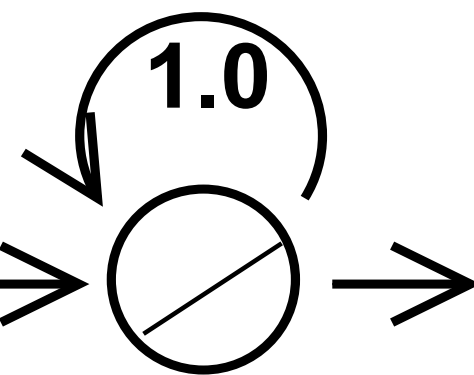
\includegraphics[width=0.25\linewidth]{images/ConstantErrorCarousel.png}
    \end{figure}
    \source{Hochreiter et al. 1997}
\end{frame}

\begin{frame}[t]{Naive Solution - Problems}
\begin{figure}
        \centering
        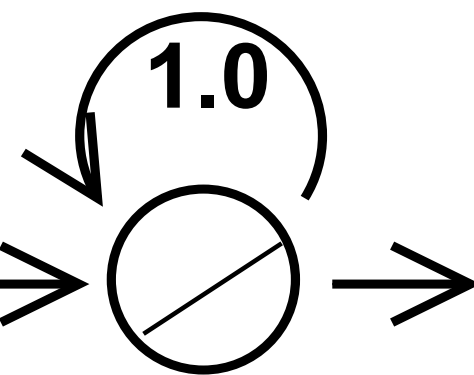
\includegraphics[width=0.25\linewidth]{images/ConstantErrorCarousel.png}
    \end{figure}
    \source{Hochreiter et al. 1997}
\end{frame}

\begin{frame}[t]{Naive Solution - Problems}
\begin{figure}
        \centering
        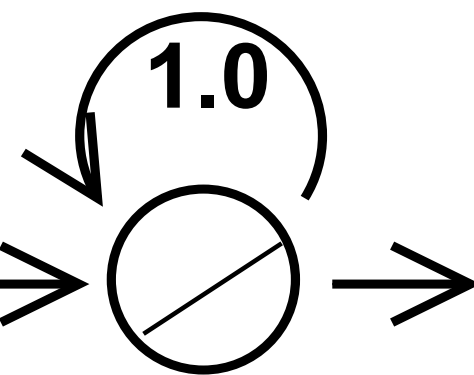
\includegraphics[width=0.25\linewidth]{images/ConstantErrorCarousel.png}
    \end{figure}
Connected to other units:
\source{Hochreiter et al. 1997}
\end{frame}

\begin{frame}[t]{Naive Solution - Problems}
\begin{figure}
        \centering
        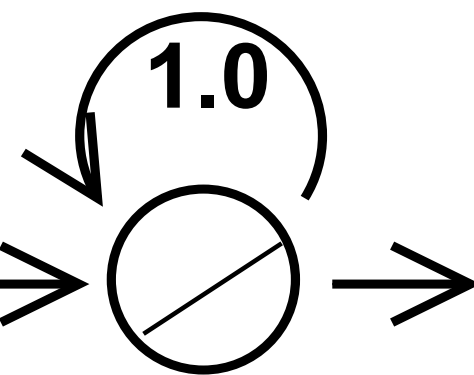
\includegraphics[width=0.25\linewidth]{images/ConstantErrorCarousel.png}
    \end{figure}
Connected to other units:
\begin{itemize}
    \item Input from unit \begin{math}i\end{math}
\end{itemize}
\source{Hochreiter et al. 1997}
\end{frame}

\begin{frame}[t]{Naive Solution - Problems}
\begin{figure}
        \centering
        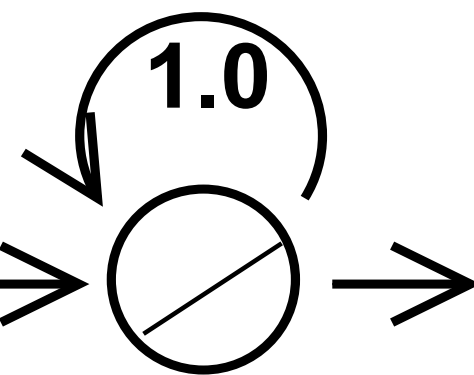
\includegraphics[width=0.25\linewidth]{images/ConstantErrorCarousel.png}
    \end{figure}
Connected to other units:
\begin{itemize}
    \item Input from unit \begin{math}i\implies\end{math}  Single weight \begin{math}w_ji\end{math} for storing \& ignoring inputs
\end{itemize}
\source{Hochreiter et al. 1997}
\end{frame}

\begin{frame}[t]{Naive Solution - Problems}
\begin{figure}
        \centering
        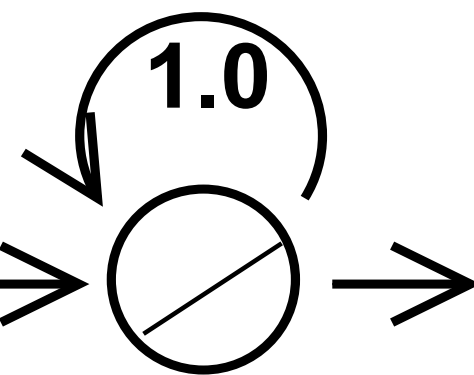
\includegraphics[width=0.25\linewidth]{images/ConstantErrorCarousel.png}
    \end{figure}
Connected to other units:
\begin{itemize}
    \item Input from unit \begin{math}i\implies\end{math} Single weight \begin{math}w_ji\end{math} for storing \& ignoring inputs
    \item Output to unit \begin{math}k\end{math}
\end{itemize}
\source{Hochreiter et al. 1997}
\end{frame}

\begin{frame}[t]{Naive Solution - Problems}
\begin{figure}
        \centering
        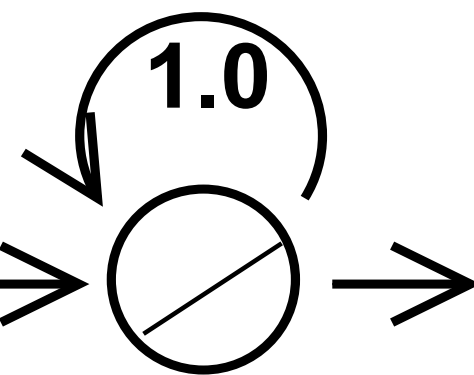
\includegraphics[width=0.25\linewidth]{images/ConstantErrorCarousel.png}
    \end{figure}
Connected to other units:
\begin{itemize}
    \item Input from unit \begin{math}i\implies\end{math} Single weight \begin{math}w_{ji}\end{math} for storing \& ignoring inputs
    
    \item Output to unit \begin{math}k\implies\end{math} Single weight \begin{math}w_{kj}\end{math} for controlling retrieval
\end{itemize}
\source{Hochreiter et al. 1997}
\end{frame}

\begin{frame}[t]{Naive Solution - Problems}
\begin{figure}
        \centering
        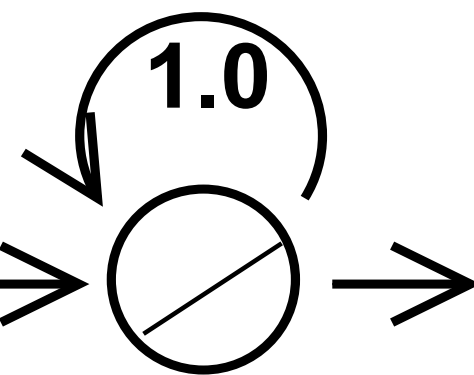
\includegraphics[width=0.25\linewidth]{images/ConstantErrorCarousel.png}
    \end{figure}
Connected to other units:
\begin{itemize}
    \item Input from unit \begin{math}i\implies\end{math} Single weight \begin{math}w_{ji}\end{math} for storing \& ignoring inputs
    
    \item Output to unit \begin{math}k\implies\end{math} Single weight \begin{math}w_{kj}\end{math} for controlling retrieval
\end{itemize}
Conflicting weight update signals for \begin{math}w_{ji}\end{math} \& \begin{math}w_{kj}\end{math}
\source{Hochreiter et al. 1997}
\end{frame}

\begin{frame}[t]{Naive Solution - Problems}
\begin{figure}
        \centering
        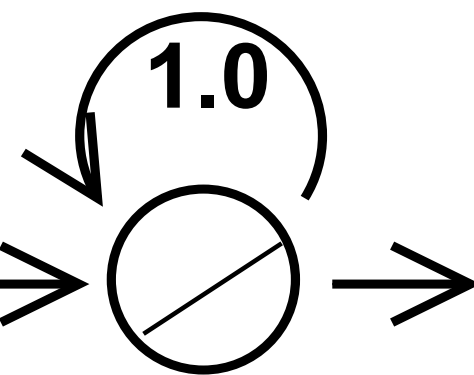
\includegraphics[width=0.25\linewidth]{images/ConstantErrorCarousel.png}
    \end{figure}
Connected to other units:
\begin{itemize}
    \item Input from unit \begin{math}i\implies\end{math} Single weight \begin{math}w_{ji}\end{math} for storing \& ignoring inputs
    
    \item Output to unit \begin{math}k\implies\end{math} Single weight \begin{math}w_{kj}\end{math} for controlling retrieval
\end{itemize}
Conflicting weight update signals for \begin{math}w_{ji}\end{math} \& \begin{math}w_{kj}\implies\end{math} Mechanism for storage and retrieval
\source{Hochreiter et al. 1997}
\end{frame}

% LSTM Architecture
\begin{frame}[t]{Contents}
\begin{itemize}
    \item Introduction
    \item Recap
    \item Naive Solution
    \item \textbf{LSTM Architecture}
    \item Variants
    \item GRU
    \item LSTM vs Transformer
    \item Applications
    \item Discussion
    \item Conclusion
\end{itemize}
\end{frame}

\begin{frame}[t]{LSTM Architecture - Gate Unit}
Idea: Restrict flow based on context
\source{Hochreiter et al. 1997}
\end{frame}

\begin{frame}[t]{LSTM Architecture - Gate Unit}
Idea: Restrict flow based on context
\begin{figure}
    \centering
    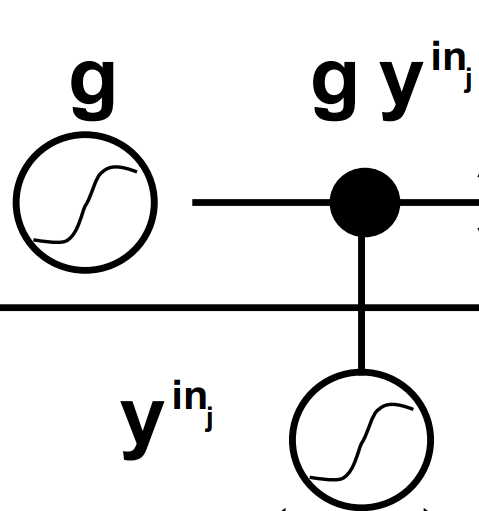
\includegraphics[width=0.2\linewidth]{images/GateUnit.png}
\end{figure}
\source{Hochreiter et al. 1997}
\end{frame}

\begin{frame}[t]{LSTM Architecture - Gate Unit}
Idea: Restrict flow based on context
\begin{figure}
    \centering
    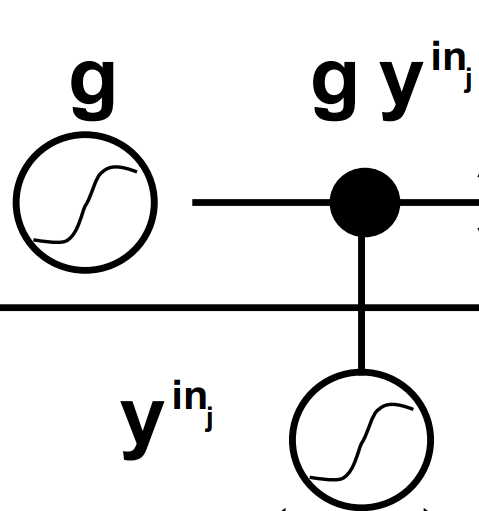
\includegraphics[width=0.2\linewidth]{images/GateUnit.png}
\end{figure}
Input gets scaled by number computed from context
\source{Hochreiter et al. 1997}
\end{frame}


\begin{frame}[t]{LSTM Architecture - Memory Cell}
Memory Cell: CEC unit with input and output gate units
\source{Hochreiter et al. 1997}
\end{frame}

\begin{frame}[t]{LSTM Architecture - Memory Cell}
Memory Cell: CEC unit with input and output gate units
\begin{figure}
    \centering
    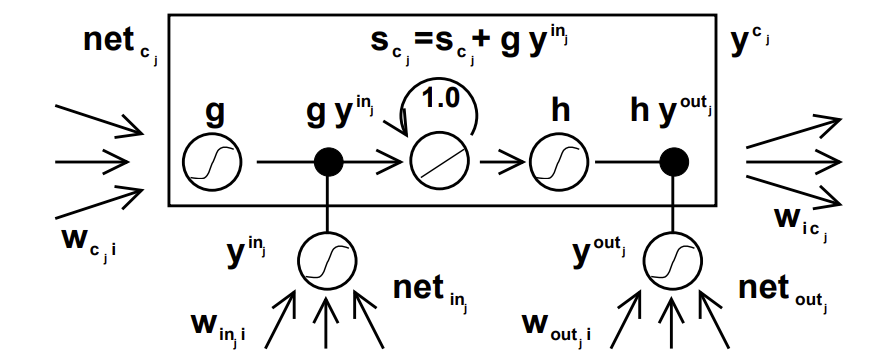
\includegraphics[width=1\linewidth]{images/LSTM-Cell-Diagram.png}
\end{figure}
\source{Hochreiter et al. 1997}
\end{frame}

\begin{frame}[t]{LSTM Architecture - Network Topology}
Inputs for cell and gates can be chosen:
\end{frame}

\begin{frame}[t]{LSTM Architecture - Network Topology}
Input for cell and gate units can be:
\begin{itemize}
    \item Input Units
\end{itemize}
\end{frame}

\begin{frame}[t]{LSTM Architecture - Network Topology}
Input for cell and gate units can be:
\begin{itemize}
    \item Input Units
    \item Gate Units
\end{itemize}
\end{frame}

\begin{frame}[t]{LSTM Architecture - Network Topology}
Input for cell and gate units can be:
\begin{itemize}
    \item Input Units
    \item Gate Units
    \item Memory Cells
\end{itemize}
\end{frame}

\begin{frame}[t]{LSTM Architecture - Network Topology}
Input for cell and gate units can be:
\begin{itemize}
    \item Input Units
    \item Gate Units
    \item Memory Cells
    \item Conventional Hidden Units
\end{itemize}
\end{frame}

\begin{frame}[t]{LSTM Architecture - Network Topology}
Input for cell and gate units can be:
\begin{itemize}
    \item Input Units
    \item Gate Units
    \item Memory Cells
    \item Conventional Hidden Units
\end{itemize}
Commonly used topology: Inputs for Cell \& Gate are all input units \& memory cell outputs
\end{frame}

\begin{frame}[t]{LSTM Architecture - Network Topology}
Input for cell and gate units can be:
\begin{itemize}
    \item Input Units
    \item Gate Units
    \item Memory Cells
    \item Conventional Hidden Units
\end{itemize}
Commonly used topology: Inputs for Cell \& Gate are all input units \& memory cell outputs
Input Gate: \begin{math}i_t=\sigma_i\left(W_{i\ h}h_{t-1}+W_{i\ x} x_t\right)\end{math}
\end{frame}

\begin{frame}[t]{LSTM Architecture - Network Topology}
Input for cell and gate units can be:
\begin{itemize}
    \item Input Units
    \item Gate Units
    \item Memory Cells
    \item Conventional Hidden Units
\end{itemize}
Commonly used topology: Inputs for Cell \& Gate are all input units \& memory cell outputs
Input Gate:  \begin{math}i_t=\sigma_i\left(W_{i\ h}h_{t-1}+W_{i\ x} x_t\right)\end{math}\\
Output Gate: \begin{math}o_t=\sigma_o\left(W_{o\ h}h_{t-1}+W_{o\ x}x_t\right)\end{math}
\end{frame}

\begin{frame}[t]{LSTM Architecture - Network Topology}
Input for cell and gate units can be:
\begin{itemize}
    \item Input Units
    \item Gate Units
    \item Memory Cells
    \item Conventional Hidden Units
\end{itemize}
Commonly used topology: Inputs for Cell \& Gate are all input units \& memory cell outputs
Input Gate:  \begin{math}i_t=\sigma_i\left(W_{i\ h}h_{t-1}+W_{i\ x} x_t + b_i\right)\end{math}\\
Output Gate: \begin{math}o_t=\sigma_o\left(W_{o\ h}h_{t-1}+W_{o\ x}x_t + b_o\right)\end{math}\\
Cell State: \begin{math}C_t=C_{t-1}+i_t\odot\sigma_c\left(W_{c\ h}h_{t-1}+W_{c\ x}x_t + b_c\right)\end{math} 
\end{frame}

\begin{frame}[t]{LSTM Architecture - Network Topology}
Input for cell and gate units can be:
\begin{itemize}
    \item Input Units
    \item Gate Units
    \item Memory Cells
    \item Conventional Hidden Units
\end{itemize}
Commonly used topology: Inputs for Cell \& Gate are all input units \& memory cell outputs
Input Gate:  \begin{math}i_t=\sigma_i\left(U_{i}h_{t-1}+W_{i} x_t + b_i\right)\end{math}\\
Output Gate: \begin{math}o_t=\sigma_o\left(U_{o}h_{t-1}+W_{o}x_t + b_o\right)\end{math}\\
Internal State: \begin{math}C_t=C_{t-1}+i_t\odot\sigma_c\left(U_{c}h_{t-1}+W_{x}x_t + b_c\right)\end{math}\\
Output: \begin{math}h_t=o_t\odot\sigma_h\left(C_t\right)\end{math}
\end{frame}


\begin{frame}[t]{LSTM Architecture - Limitations}
Drawbacks:
\end{frame}

\begin{frame}[t]{LSTM Architecture - Limitations}
Drawbacks:
\begin{itemize}
    \item Exploding Gradients
\end{itemize}
\end{frame}

\begin{frame}[t]{LSTM Architecture - Limitations}
Drawbacks:
\begin{itemize}
    \item Exploding Gradients
    \item Computational Intensity
\end{itemize}
\end{frame}

\begin{frame}[t]{LSTM Architecture - Limitations}
Drawbacks:
\begin{itemize}
    \item Exploding Gradients
    \item Computational Intensity
    \item Limited GPU utilization
\end{itemize}
\end{frame}

\begin{frame}[t]{LSTM Architecture - Limitations}
Drawbacks:
\begin{itemize}
    \item Exploding Gradients
    \item Computational Intensity
    \item Limited GPU utilization
    \item Memory bottlenecks
\end{itemize}
\end{frame}

\begin{frame}[t]{LSTM Architecture - Limitations}
Drawbacks:
\begin{itemize}
    \item Exploding Gradients
    \item Computational Intensity
    \item Limited GPU utilization
    \item Memory bottlenecks
    \item Worse Performance on Short Sequences
\end{itemize}
\end{frame}

\begin{frame}[t]{LSTM Architecture - Limitations}
Drawbacks:
\begin{itemize}
    \item Exploding Gradients
    \item Computational Intensity
    \item Limited GPU Utilization
    \item Memory Bottlenecks
    \item Worse performance on short sequences
    \item State can not be reset
\end{itemize}
\end{frame}


% LSTM Variants
\begin{frame}[t]{Contents}
\begin{itemize}
    \item Introduction
    \item Recap
    \item Naive Solution
    \item LSTM Architecture
    \item \textbf{Variants}
    \item GRU
    \item LSTM vs Transformer
    \item Applications
    \item Discussion
    \item Conclusion
\end{itemize}
\end{frame}

\begin{frame}[t]{Variants - LSTM with forget gate}
\begin{figure}
    \centering
    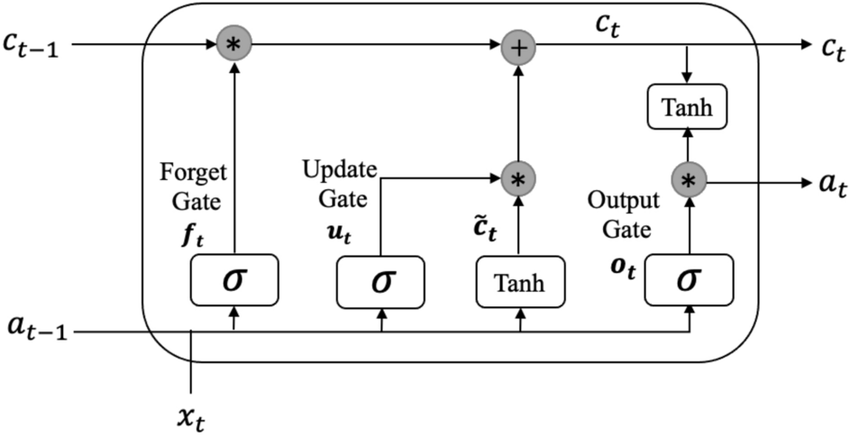
\includegraphics[width=0.75\linewidth]{images/Structure-of-LSTM-cell-which-introduces-three-special-gates-Input-Gate-i-Forget-Gate.png}
\end{figure}
\source{Nguyen et al. 2022}
\end{frame}

\begin{frame}[t]{Variants - LSTM with forget gate}
Forget Gate:
\source{Gers et al. 1999}
\end{frame}

\begin{frame}[t]{Variants - LSTM with forget gate}
Forget Gate:
\begin{itemize}
    \item "Forgetting" by resetting state
\end{itemize}
\source{Gers et al. 1999}
\end{frame}

\begin{frame}[t]{Variants - LSTM with forget gate}
Forget Gate:
\begin{itemize}
    \item "Forgetting" by resetting state
    \item Achieved by gating the previous state
\end{itemize}
\source{Gers et al. 1999}
\end{frame}

\begin{frame}[t]{Variants - LSTM with forget gate}
Forget Gate:
\begin{itemize}
    \item "Forgetting" by resetting state
    \item Achieved by gating the previous state
    \item \begin{math}f_t=\sigma_i\left(U_{f}h_{t-1}+W_{f} x_t + b_f\right)\end{math}
\end{itemize}
\source{Gers et al. 1999}
\end{frame}

\begin{frame}[t]{Variants - LSTM with forget gate}
Forget Gate:
\begin{itemize}
    \item "Forgetting" by resetting state
    \item Achieved by gating the previous state
    \item \begin{math}f_t=\sigma_i\left(U_{f}h_{t-1}+W_{f} x_t + b_f\right)\end{math}
    \item \begin{math}C_t=f_t\odot C_{t-1}+i_t\odot\sigma_c\left(U_{c}h_{t-1}+W_{x}x_t + b_c\right)\end{math}
\end{itemize}
\source{Gers et al. 1999}
\end{frame}


%GRU
\begin{frame}[t]{Contents}
\begin{itemize}
    \item Introduction
    \item Recap
    \item Naive Solution
    \item LSTM Architecture
    \item Variants
    \item \textbf{GRU}
    \item LSTM vs Transformer
    \item Applications
    \item Discussion
    \item Conclusion
\end{itemize}
\end{frame}

\begin{frame}[t]{GRU}

\end{frame}

% LSTM vs Transformer
\begin{frame}[t]{Contents}
\begin{itemize}
    \item Introduction
    \item Recap
    \item Naive Solution
    \item LSTM Architecture
    \item Variants
    \item GRU
    \item \textbf{LSTM vs Transformer}
    \item Applications
    \item Discussion
    \item Conclusion
\end{itemize}
\end{frame}

\begin{frame}[t]{LSTM vs Transformers}
    
\end{frame}

%LSTM Applications
\begin{frame}[t]{Contents}
\begin{itemize}
    \item Introduction
    \item Recap
    \item Naive Solution
    \item LSTM Architecture
    \item Variants
    \item GRU
    \item LSTM vs Transformer
    \item \textbf{Applications}
    \item Discussion
    \item Conclusion
\end{itemize}
\end{frame}
%Time Series Forecasting
\begin{frame}[t]{Applications - Time Series Forecasting}
LSTMs perform better on:
\end{frame}

\begin{frame}[t]{Applications - Time Series Forecasting}
LSTMs perform better on:
\begin{itemize}
    \item Long sequences
\end{itemize}
\end{frame}

\begin{frame}[t]{Applications - Time Series Forecasting}
LSTMs perform better on:
\begin{itemize}
    \item Long sequences
    \item Complex sequences
\end{itemize}
\end{frame}

\begin{frame}[t]{Applications - Time Series Forecasting}
LSTMs perform better on:
\begin{itemize}
    \item Long sequences
    \item Complex sequences
\end{itemize}
Examples:
\end{frame}

\begin{frame}[t]{Applications - Time Series Forecasting}
LSTMs perform better on:
\begin{itemize}
    \item Long sequences
    \item Complex sequences
\end{itemize}
Examples:
\begin{itemize}
    \item 2022: Deep LSTM Network forecasts electricity demand (1.5\% accuracy)
\end{itemize}
\end{frame}

\begin{frame}[t]{Applications - Time Series Forecasting}
LSTMs perform better on:
\begin{itemize}
    \item Long sequences
    \item Complex sequences
\end{itemize}
Examples:
\begin{itemize}
    \item 2022: Deep LSTM Network forecasts electricity demand (1.5\% accuracy)
    \item 2024: LSTM Architecture forcasts electricity prices 
\end{itemize}
\end{frame}

%Music Generation
\begin{frame}[t]{Applications - Music Generation}
Music has temporal structure:
\end{frame}

\begin{frame}[t]{Applications - Music Generation}
Music has temporal structure:
\begin{itemize}
    \item Rhythms
\end{itemize}
\end{frame}

\begin{frame}[t]{Applications - Music Generation}
Music has temporal structure:
\begin{itemize}
    \item Rhythms
    \item Chord progressions
\end{itemize}
\end{frame}

\begin{frame}[t]{Applications - Music Generation}
Music has temporal structure:
\begin{itemize}
    \item Rhythms
    \item Chord progressions
    \item Melodic motives
\end{itemize}
\end{frame}

\begin{frame}[t]{Applications - Music Generation}
Music has temporal structure:
\begin{itemize}
    \item Rhythms
    \item Chord progressions
    \item Melodic motives
\end{itemize}
Easily representable as numbers
\end{frame}

\begin{frame}[t]{Applications - Music Generation}
Music has temporal structure:
\begin{itemize}
    \item Rhythms
    \item Chord progressions
    \item Melodic motives
\end{itemize}
Easily representable as numbers\\
2002: LSTM Architecture used to compose music
\end{frame}

%Discussion
\begin{frame}[t]{Contents}
\begin{itemize}
    \item Introduction
    \item Recap
    \item Naive Solution
    \item LSTM Architecture
    \item Variants
    \item GRU
    \item LSTM vs Transformer
    \item Applications
    \item \textbf{Discussion}
    \item Conclusion
\end{itemize}
\end{frame}
\begin{frame}[t]{Discussion - the Future of LSTMs}
Future of the LSTM architecture:
\end{frame}

\begin{frame}[t]{Discussion - the Future of LSTMs}
Future of the LSTM architecture:
\begin{itemize}
    \item Largely replaced by transformers
\end{itemize}
\end{frame}


\begin{frame}[t]{Discussion - the Future of LSTMs}
Future of the LSTM architecture:
\begin{itemize}
    \item Largely replaced by transformers
    \begin{itemize}
        \item LSTMs still useful for small datasets (better performance)
    \end{itemize} 
\end{itemize}
\end{frame}

\begin{frame}[t]{Discussion - the Future of LSTMs}
Future of the LSTM architecture:
\begin{itemize}
    \item Largely replaced by transformers
    \begin{itemize}
        \item LSTMs still useful for small datasets (better performance)
        \item LSTM - Transformer hybrid architectures 
    \end{itemize} 
\end{itemize}
\end{frame}

\begin{frame}[t]{Discussion - the Future of LSTMs}
Future of the LSTM architecture:
\begin{itemize}
    \item Largely replaced by transformers
    \begin{itemize}
        \item LSTMs still useful for small datasets (better performance)
        \item LSTM - Transformer hybrid architectures 
    \end{itemize} 
    \item Inspired many RNN Architectures
\end{itemize}
\end{frame}

%Conclusion
\begin{frame}[t]{Conclusion}
LSTM Architecture:
\end{frame}


\begin{frame}[t]{Conclusion}
LSTM Architecture:
\begin{itemize}
    \item Internal CEC unit \begin{math}\implies \end{math} Internal State (Memory)
\end{itemize}
\end{frame}

\begin{frame}[t]{Conclusion}
LSTM Architecture:
\begin{itemize}
    \item Internal CEC unit \begin{math}\implies \end{math} Internal State (Memory)
    \item Input Gate \begin{math}\implies\end{math} Protects memory from unwanted perturbation
\end{itemize}
\end{frame}

\begin{frame}[t]{Conclusion}
LSTM Architecture:
\begin{itemize}
    \item Internal CEC unit \begin{math}\implies \end{math} Internal State (Memory)
    \item Input Gate \begin{math}\implies\end{math} Protects memory from unwanted perturbation
    \item Output Gate \begin{math}\implies\end{math} Controls output of the memory to other units
\end{itemize}
\end{frame}

\begin{frame}[t]{Conclusion}
LSTM Architecture:
\begin{itemize}
    \item Internal CEC unit \begin{math}\implies \end{math} Internal State (Memory)
    \item Input Gate \begin{math}\implies\end{math} Protects memory from unwanted perturbation
    \item Output Gate \begin{math}\implies\end{math} Controls output of the memory to other units
    \item \begin{math}\implies\end{math} Eliminates vanishing Gradient Problem
\end{itemize}
\end{frame}

\begin{frame}[t]{Conclusion}
LSTM Architecture:
\begin{itemize}
    \item Internal CEC unit \begin{math}\implies \end{math} Internal State (Memory)
    \item Input Gate \begin{math}\implies\end{math} Protects memory from unwanted perturbation
    \item Output Gate \begin{math}\implies\end{math} Controls output of the memory to other units
    \item \begin{math}\implies\end{math} Eliminates vanishing Gradient Problem
    \item Historically important 
\end{itemize}
\end{frame}

\begin{frame}[t]{Conclusion}
LSTM Architecture:
\begin{itemize}
    \item Internal CEC unit \begin{math}\implies \end{math} Internal State (Memory)
    \item Input Gate \begin{math}\implies\end{math} Protects memory from unwanted perturbation
    \item Output Gate \begin{math}\implies\end{math} Controls output of the memory to other units
    \item \begin{math}\implies\end{math} Eliminates vanishing Gradient Problem
    \item Historically important 
    \item Inspired many RNN Architectures
\end{itemize}
Currently:
\end{frame}

\begin{frame}[t]{Conclusion}
LSTM Architecture:
\begin{itemize}
    \item Internal CEC unit \begin{math}\implies \end{math} Internal State (Memory)
    \item Input Gate \begin{math}\implies\end{math} Protects memory from unwanted perturbation
    \item Output Gate \begin{math}\implies\end{math} Controls output of the memory to other units
    \item \begin{math}\implies\end{math} Eliminates vanishing Gradient Problem
    \item Historically important 
    \item Inspired many RNN Architectures
\end{itemize}
Currently:
\begin{itemize}
    \item Replaced by transformers
\end{itemize}
\end{frame}

\begin{frame}[t]{Conclusion}
LSTM Architecture:
\begin{itemize}
    \item Internal CEC unit \begin{math}\implies \end{math} Internal State (Memory)
    \item Input Gate \begin{math}\implies\end{math} Protects memory from unwanted perturbation
    \item Output Gate \begin{math}\implies\end{math} Controls output of the memory to other units
    \item \begin{math}\implies\end{math} Eliminates vanishing Gradient Problem
    \item Historically important 
    \item Inspired many RNN Architectures
\end{itemize}
Currently:
\begin{itemize}
    \item Replaced by transformers
    \item Development of new LSTM based architectures
\end{itemize}
\end{frame}

\begin{frame}[t]{Conclusion}
LSTM Architecture:
\begin{itemize}
    \item Internal CEC unit \begin{math}\implies \end{math} Internal State (Memory)
    \item Input Gate \begin{math}\implies\end{math} Protects memory from unwanted perturbation
    \item Output Gate \begin{math}\implies\end{math} Controls output of the memory to other units
    \item \begin{math}\implies\end{math} Eliminates vanishing Gradient Problem
    \item Historically important 
    \item Inspired many RNN Architectures
\end{itemize}
Currently:
\begin{itemize}
    \item Replaced by transformers
    \item Development of new LSTM based architectures
    \item Remain useful in some cases
\end{itemize}
\end{frame}

% ----------------------------------------------------------------
\nocite{alselwi2024lstmfuture}
\nocite{bolboaca2023lstmperformance}
\nocite{eck2002musicgeneration}
\nocite{gers1999forgetgate}
\nocite{gers2001timeseries}
\nocite{gokmen2018hadamard}
\nocite{gradient-clipping}
\nocite{harris1954languagestructure}
\nocite{hochreiter1997lstm}
\nocite{nielsen2024electricitypriceforcasting}
\nocite{torres2022elctricityforecasting}
\nocite{zhao2025lstmtransformerhybrid}
\nocite{zheng2018scalability}
\nocite{zheng2020scalability}

\setbeamerfont{bibliography item}{size=\footnotesize}
\setbeamerfont{bibliography entry author}{size=\footnotesize}
\setbeamerfont{bibliography entry title}{size=\footnotesize}
\setbeamerfont{bibliography entry location}{size=\footnotesize}
\setbeamerfont{bibliography entry note}{size=\footnotesize}
\begin{frame}[allowframebreaks]{References}

  \bibliographystyle{alpha}
  \bibliography{slides}

\end{frame}
\end{document}